% Cours3 - Méthode des éléments finis en pratique

\documentclass[
mode=present,    % "present" or "print" (pas de overlays,etc.) or "handout" (2slides/page)
paper=a4paper,   % "screen" or "a4paper" or "smartboard" (widescreen)
orient=landscape,
display=slides,   % "slides" or "slidesnotes" or "notes"
size=10pt,     % default=11pt
style=romain   % default, simple, fyma, ciment, horatio, paintings, jefka, ...
]{powerdot}

\usepackage{mypdotstyle}

\graphicspath{ {cours03/fig/} }   % includegraphics
\lstset{inputpath=cours03}        % listings

\pdsetup{
cf={MATH0471 -- Cours 3}, % centre footer
lf={ULg, Liège, Belgium}, % left footer
trans=Replace,  % Split, Blinds, Box, Wipe, Dissolve, Glitter, Replace
  }

\begin{document}

    % reduction of the space before and after equations
    % (must be after "\begin{document}")
    \setlength{\belowdisplayskip}{2pt}
    \setlength{\belowdisplayshortskip}{2pt}
    \setlength{\abovedisplayskip}{2pt}
    \setlength{\abovedisplayshortskip}{2pt}

\title{\vspace{-5mm}
         {\sl\small MATH0471 -- Projet de calcul scientifique multiphysique} \\
        \vspace{5mm}
        \Large Méthode des éléments finis en pratique\\
        \vspace{5mm}
}
\author{R. Boman \& C. Geuzaine}
\date{\today}
\maketitle

%=======================================================================
% TABLE DES MATIERES
%=======================================================================

\begin{slide}[toc=,bm=]{Table des matières}
\tableofcontents[content=sections] % sections, all
\end{slide}
%=======================================================================



%=======================================================================
\section[toc=Rappels MEF]{Rappel sur la Méthode des Éléments Finis (MEF)}
%=======================================================================

%-----------------------------------------------------------------------
\begin{slide}{Problème à résoudre}
%-----------------------------------------------------------------------

Soit l'EDP suivante à résoudre sur le domaine spatial 3D $\Omega$:
\begin{equation*}
    \Delta u = f(\boldsymbol{x})
\end{equation*}
où $u=u(\boldsymbol{x})$ est un champ scalaire.

\begin{center}
    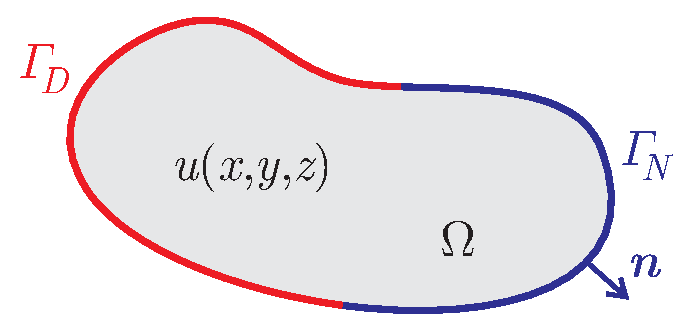
\includegraphics[width=0.5\textwidth]{dom.eps}
\end{center}

L'équation est accompagnée de conditions aux limites de Dirichlet
\begin{equation*}
    u = u_D \qquad \text{ sur } \Gamma_D
\end{equation*}
et de conditions aux limites de Neumann
\begin{equation*}
    \boldsymbol{\nabla} u . \boldsymbol{n} = g \qquad \text{ sur } \Gamma_N
\end{equation*}

\end{slide}

%-----------------------------------------------------------------------
\begin{slide}{Forme variationnelle}
%-----------------------------------------------------------------------

Une forme variationnelle est obtenue en multipliant l'EDP par une fonction test $h(\boldsymbol{x})$ et en intégrant sur le volume $\Omega$:
\begin{equation*}
     \int_{\Omega}h\, \Delta u \,d\Omega = \int_{\Omega} h\, f \,d\Omega
\end{equation*}
L'équation résultante est ensuite intégrée par parties:
\begin{equation*}
     \boxed{
     \int_{\Gamma_D \cup \Gamma_N} h\, \boldsymbol{\nabla} u \cdot \boldsymbol{n} \,d\Gamma
          - \int_{\Omega} \boldsymbol{\nabla} h \cdot \boldsymbol{\nabla} u \,d\Omega
     =
     \int_{\Omega} h\, f \,d\Omega
     }
\end{equation*}

\vspace{1cm}

Le premier terme se décompose en:
\begin{equation*}
     \int_{\Gamma_D \cup \Gamma_N} h\, \boldsymbol{\nabla} u \cdot \boldsymbol{n} \,d\Gamma
          =
      \underbrace{\int_{\Gamma_D}h\, \boldsymbol{\nabla} u \cdot \boldsymbol{n} \,d\Gamma}_{= 0 \text{ si $h=0$ sur $\Gamma_D$}}
      +
    \int_{\Gamma_N} h\,\underbrace{\boldsymbol{\nabla} u \cdot \boldsymbol{n}}_{ = g \text{ (C.L.)} } \,d\Gamma
\end{equation*}
On se restreint donc à des fonctions tests $h(\boldsymbol{x})$ qui s'annulent sur $\Gamma_D$.

\end{slide}


%-----------------------------------------------------------------------
\begin{slide}[toc=]{Forme variationnelle}
%-----------------------------------------------------------------------

Une forme variationnelle du problème peut s'écrire:

\bigskip

\noindent\fbox{\parbox{\linewidth-2\fboxrule-2\fboxsep}{ %-----------------------------------------------------------
Etant donné une fonction $f$ de $L^2(\Omega)$, trouver une fonction $u$ de $H^1(\Omega)$ qui vérifie $u=u_D$ sur $\Gamma_D$ telle que:
\begin{equation*}
     \int_{\Gamma_N} h\,g \,d\Gamma
          - \int_{\Omega} \boldsymbol{\nabla} h \cdot \boldsymbol{\nabla} u \,d\Omega
     =
     \int_{\Omega} h\, f \,d\Omega
\end{equation*}
pour toutes les fonctions tests $h$ dans $H^1(\Omega)$ telles que $h=0$ sur $\Gamma_D$.
}} %-----------------------------------------------------------------------------------------------------------------

\vspace{\stretch{1}}

Pour plus d'info, voir cours ULg:
\begin{itemize}
\item \href{http://progcours.ulg.ac.be/cocoon/cours/MATH0024-1.html}{MATH0024} - Partial Differential Equations (M. Arnst)
\item \href{http://progcours.ulg.ac.be/cocoon/cours/MECA0036-1.html}{MECA0036} - Finite Element Method (J.-P. Ponthot)
\item etc.
\end{itemize}

\end{slide}


%-----------------------------------------------------------------------
\begin{slide}{Approximation de Galerkin}
%-----------------------------------------------------------------------

Au lieu de résoudre le problème précédent, on définit une base de $N$ fonctions $\varphi_j(\boldsymbol{x})$ sur $\Omega$ et on recherche une solution $u$ de la formulation variationnelle parmi les fonctions $u$ qui sont des combinaisons linéaires de des $\varphi_j$:

\begin{equation*}
     u^*(\boldsymbol{x}) = \sum_{j=1}^N u_j \,\varphi_j(\boldsymbol{x})
\end{equation*}

On se limite également aux fonctions tests qui sont des combinaisons linéaires de ces mêmes fonctions $\varphi$:

\begin{equation*}
     h^*(\boldsymbol{x}) = \sum_{i=1}^N h_i \,\varphi_i(\boldsymbol{x})
\end{equation*}

\bigskip

L'équation est discrétisée~: au lieu de rechercher une fonction continue $u(\boldsymbol{x})$, on recherche les $N$ valeurs des $u_j$.

\end{slide}


%-----------------------------------------------------------------------
\begin{slide}[toc=]{Approximation de Galerkin}
%-----------------------------------------------------------------------

Dans le cas de notre exemple, l'approximation de Galerkin s'écrit:

\bigskip

\noindent\fbox{\parbox{\linewidth-2\fboxrule-2\fboxsep}{ %-----------------------------------------------------------
Etant donné une fonction $f$ de $L^2(\Omega)$, trouver une fonction $u^*=\sum_j u_j \,\varphi_j$ qui vérifie $u^*=u_D$ sur $\Gamma_D$ telle que:
\begin{equation*}
     \int_{\Gamma_N} h^*\,g \,d\Gamma
          - \int_{\Omega} \boldsymbol{\nabla} h^* \cdot \boldsymbol{\nabla} u^* \,d\Omega
     =
     \int_{\Omega} h^*\, f \,d\Omega
\end{equation*}
pour toutes les fonctions tests $h^*=\sum_i h_i \,\varphi_i$ telles que $h^*=0$ sur $\Gamma_D$.
}} %-----------------------------------------------------------------------------------------------------------------

\bigskip

En pratique:
\begin{itemize}
\item On choisit des fonctions $\varphi_i(\boldsymbol{x})$.
\item L'équation précédente peut s'écrire sous la forme d'une combinaison linéaire de $h_i$ qui vaut 0.
\item Les $N$ coefficients des $h_i$ s'écrivent sous forme d'une expression en $u_j$.
\item Annuler cette combinaison linéaire en $h_i$, revient à annuler chaque coefficient.
\item On résout le système de $N$ équations (1 équation pour chaque $h_i$) à $N$ inconnues (les $u_j$).
\end{itemize}

\end{slide}



%-----------------------------------------------------------------------
\begin{slide}{Éléments Finis}
%-----------------------------------------------------------------------

Une méthode élément fini correspond à un choix particulier de fonctions $\varphi_i$ sur le domaine spatial $\Omega$.

\bigskip

Pour définir ces fonctions $\varphi_i$, on découpe le domaine $\Omega$ en sous-domaines de géométrie simple (quadrangles, hexaèdres) grâce à un mailleur (p. expl. \href{http://geuz.org/gmsh/}{gmsh}).

    \centerline{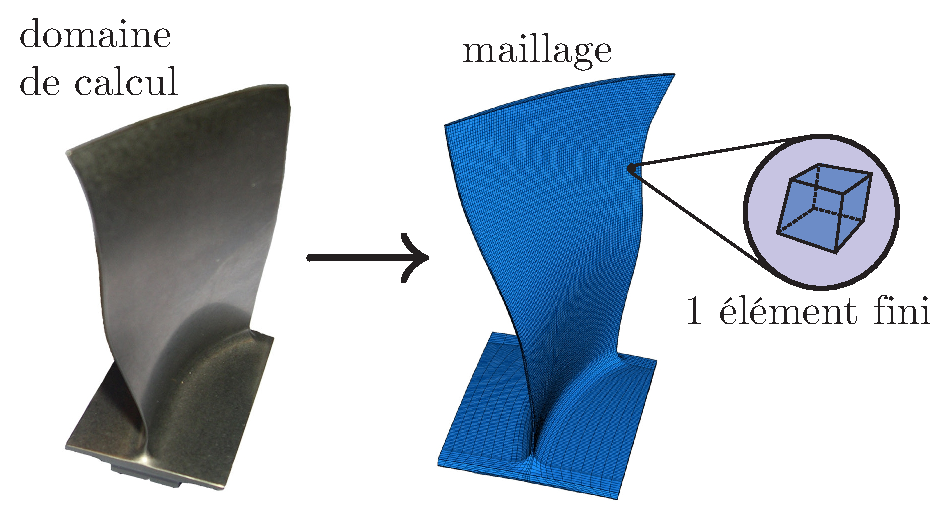
\includegraphics[width=0.65\textwidth]{blade.eps} }

Les mailles générées sont appelées \textbf{éléments finis} dans le cadre de la méthode.

\end{slide}

%=======================================================================
\section[toc=Exemple: EF 1D]{Exemple: Éléments Finis 1D}
%=======================================================================


%-----------------------------------------------------------------------
\begin{slide}{Maillage 1D}
%-----------------------------------------------------------------------

Pour comprendre intuitivement le principe de la méthode des éléments finis, on considère tout d'abord un problème à une seule dimension. L'extension 3D sera faite par la suite.
\bigskip

A 1D, le domaine $\Omega$ est divisé en segments.

\bigskip

    \centerline{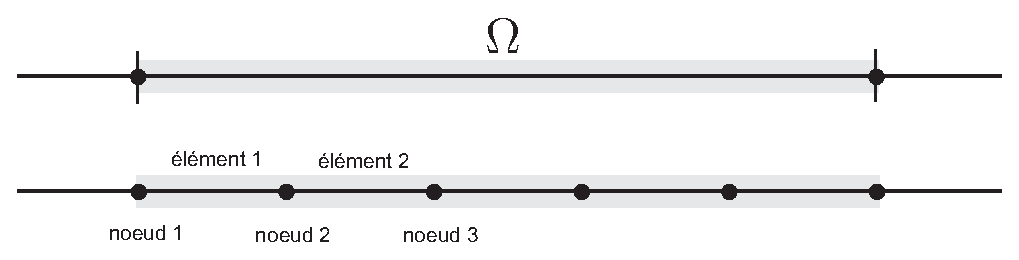
\includegraphics[width=0.8\textwidth]{mesh1d.eps} }

\bigskip

Chaque point du maillage est un noeud.

Chaque segment du maillage est un élément fini.

\end{slide}

%-----------------------------------------------------------------------
\begin{slide}{Fonctions tests}
%-----------------------------------------------------------------------

Dans le cadre de ce cours, les fonctions $\varphi_i(x)$ sont choisies linéaires par morceaux (on parle d'éléments finis linéaires). Les $\varphi_i(x)$ valent 1 au noeud $i$ et 0 aux autres noeuds.

\bigskip

    \centerline{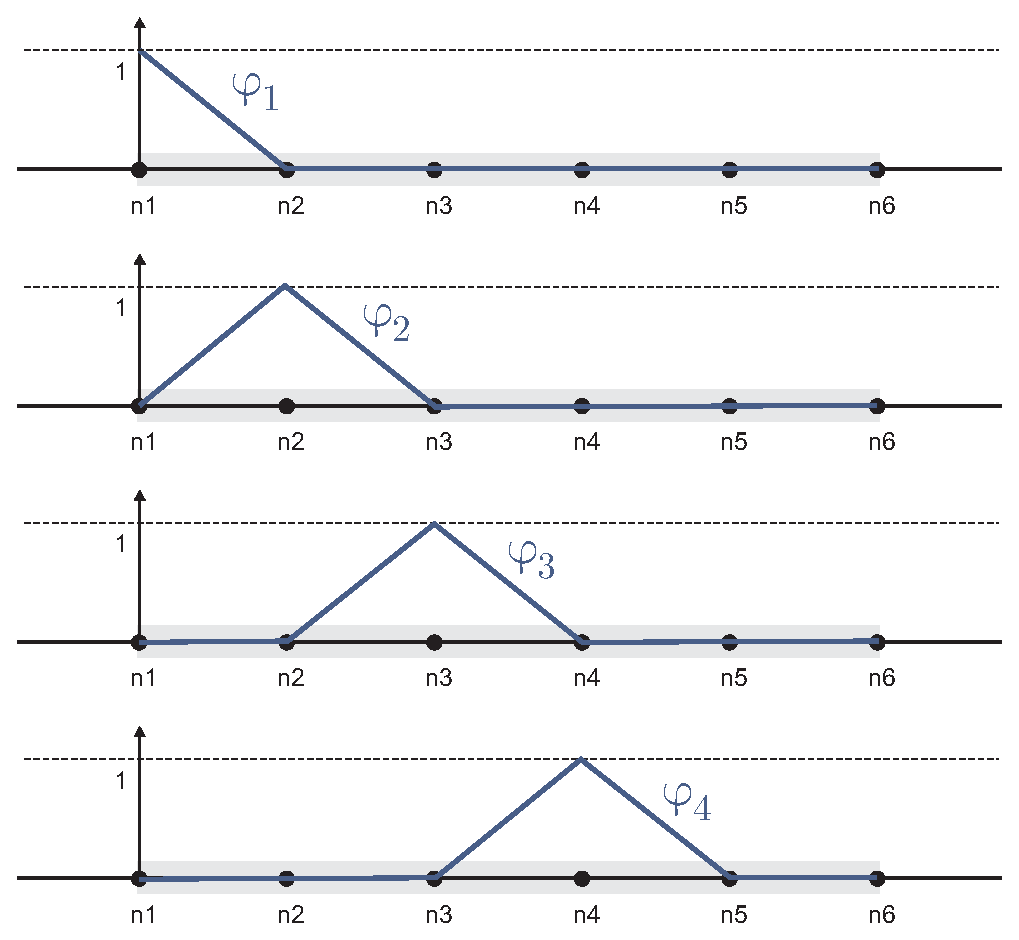
\includegraphics[width=0.55\textwidth]{phi1d.eps} }

\end{slide}

%-----------------------------------------------------------------------
\begin{slide}{Cas de Laplace}
%-----------------------------------------------------------------------

Retour à l'approximation de Galerkin. Considérons le cas de l'équation de Laplace (EDP précédente où $f=0$) avec conditions aux limites de Dirichlet ($\Gamma_N=\emptyset$). On a, dans ce cas particulier:

\begin{equation*}
    \int_{\Omega} \boldsymbol{\nabla} h^* \cdot \boldsymbol{\nabla} u^* \,d\Omega
     = 0
\end{equation*}

\bigskip

En remplaçant $h^*$ et $u^*$:
\begin{equation*}
    \int_0^L \frac{\partial}{\partial x} \left( \sum_{i=0}^N h_i\, \varphi_i(x) \right)
    \frac{\partial}{\partial x} \left( \sum_{j=0}^N u_j\, \varphi_j(x) \right) \, dx
     = 0
\end{equation*}
où $L$ est la taille du domaine $\Omega$.

\bigskip

Puisque $u_i$ et $h_j$ ne dépendent pas de $x$:
\begin{equation*}
    \int_0^L \left( \sum_{i=0}^N h_i\,\frac{\partial\varphi_i(x)}{\partial x} \right)
    \left( \sum_{j=0}^N u_j\, \frac{\partial\varphi_j(x)}{\partial x} \right) \, dx
     = 0
\end{equation*}


\end{slide}



%-----------------------------------------------------------------------
\begin{slide}[toc=]{Cas de Laplace}
%-----------------------------------------------------------------------


C'est-à-dire:
\begin{equation*}
    \sum_{i=0}^N \left[ \sum_{j=0}^N\underbrace{\left( \int_0^L \frac{\partial\varphi_i(x)}{\partial x}
    \frac{\partial\varphi_j(x)}{\partial x}  \, dx \right)}_{K_{ij}} \, u_j \right] \,  h_i
     = 0
\end{equation*}

\bigskip

On retrouve bien une combinaison linéaire des $h_i$. Celle-ci est nulle pour tout $h_i$ si les coefficients sont nuls. Autrement dit:

\begin{equation*}
\sum_{j=0}^N K_{ij} \, u_j = 0     \qquad (i=2,N-1)
\end{equation*}

Dans le cas de cette EDP, on obtient donc un système linéaire à résoudre pour obtenir les valeurs nodales $u_j$ de la solution.

\end{slide}


%-----------------------------------------------------------------------
\begin{slide}[toc=]{Cas de Laplace}
%-----------------------------------------------------------------------

\emph{Conditions aux limites}

\bigskip

Sur la frontière du domaine ($x=0$ et $x=L$), nous avons défini des conditions aux limites de Dirichlet:

\begin{equation*}
    \begin{aligned}
     u=u_0 & \qquad \text{ en } x=0 \\
     u=u_L & \qquad \text{ en } x=L \\
    \end{aligned}
\end{equation*}

\bigskip

La formulation variationnelle spécifie que $h_i=0$ sur la frontière. Les équations $i=1$ et $i=N$ sont simplement remplacées par les deux équations ci-dessus.


\end{slide}

%-----------------------------------------------------------------------
\begin{slide}[toc=]{Cas de Laplace}
%-----------------------------------------------------------------------

Calcul de la matrice $[K]$

\begin{equation*}
    K_{ij} = \int_0^L \frac{\partial\varphi_i(x)}{\partial x}
    \frac{\partial\varphi_j(x)}{\partial x}  \, dx
\end{equation*}

Si on a $N_e$ éléments finis, l'intégrale sur le domaine $\Omega$ va être calculée comme la somme des intégrales sur chaque élément.

\begin{equation*}
    K_{ij} = \int_0^L (\star)  \, dx = \sum_{e=1}^{N_e} \underbrace{\left( \int_{E_e} (\star)  \, dx \right)}_{K_{ij}^e}
\end{equation*}

\bigskip

En pratique:
\begin{itemize}
\item On calcule la contribution de l'élément $e$ ($[K^e]$ est appelée matrice ``élémentaire'').
\item On ``assemble'' (on somme) la matrice élémentaire $[K^e]$ dans la matrice globale du problème $[K]$.
\end{itemize}

\end{slide}




%-----------------------------------------------------------------------
\begin{slide}{Calcul de $[K^e]$}
%-----------------------------------------------------------------------

Pour calculer la matrice $[K^e]$

\begin{equation*}
    K^e_{ij} = \int_{E^e} \frac{\partial\varphi_i(x)}{\partial x}
    \frac{\partial\varphi_j(x)}{\partial x}  \, dx
\end{equation*}

\bigskip

on se focalise sur un seul élément fini:

\begin{center}
    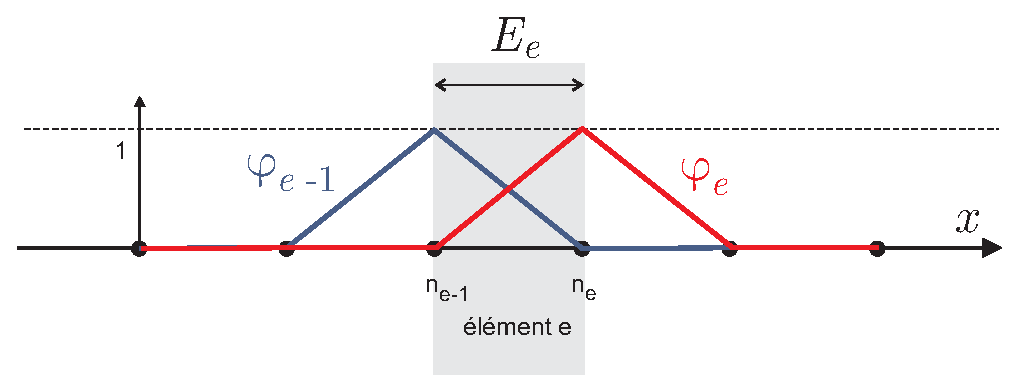
\includegraphics[width=0.8\textwidth]{Ke1.eps}
\end{center}

et on oublie momentanément le reste...

\end{slide}



%-----------------------------------------------------------------------
\begin{slide}[toc=]{Calcul de $[K^e]$}
%-----------------------------------------------------------------------

L'élément possède 2 noeuds, on les renomme localement $n_1$ et $n_2$ (respectivement de coordonnées $x_1$ et $x_2$).

L'élément ``voit'' deux fonctions $\varphi(x)$, on les renomme $\varphi_1$ et $\varphi_2$.

\bigskip

    \centerline{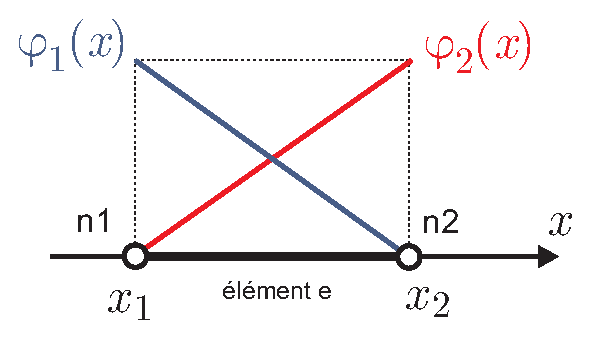
\includegraphics[width=0.4\textwidth]{Ke2.eps} }


\begin{equation*}
    \left\{
    \begin{aligned}
        &\varphi_1(x) = \frac{x-x_2}{x_1-x_2} \\
        &\varphi_2(x) = \frac{x-x_1}{x_2-x_1}
    \end{aligned}
    \right.
\end{equation*}


On doit calculer:
\begin{equation*}
    K^e_{ij} = \int_{x_1}^{x_2} \frac{\partial\varphi_i(x)}{\partial x}
    \frac{\partial\varphi_j(x)}{\partial x}  \, dx
\end{equation*}

\end{slide}

%-----------------------------------------------------------------------
\begin{slide}[toc=]{Calcul de $[K^e]$}
%-----------------------------------------------------------------------

Pour calculer l'intégrale, on peut effectuer un changement de variable $x\in[x_1,x_2] \rightarrow \xi\in[-1,1]$.
    \centerline{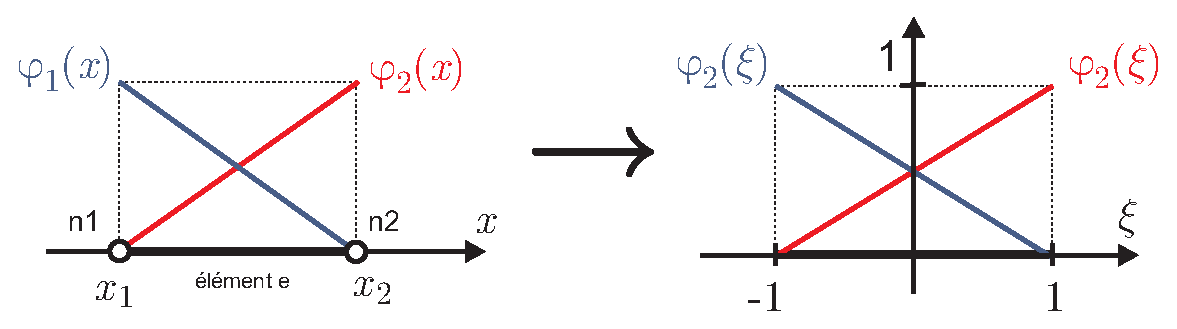
\includegraphics[width=0.8\textwidth]{Ke3.eps} }
On a:
\begin{equation*}
    \left\{
        \begin{aligned}
            &\varphi_1(\xi) = \frac{1}{2} (1-\xi) \\
            &\varphi_2(\xi) = \frac{1}{2} (1+\xi)
        \end{aligned}
    \right.
\end{equation*}
et
\begin{equation*}
    x(\xi) = \frac{1-\xi}{2} x_1 + \frac{1+\xi}{2} x_2
    = \varphi_1(\xi) x_1 +  \varphi_2(\xi) x_2
    = \sum_{i=1}^2 \varphi_i(\xi) x_i
\end{equation*}

\end{slide}


%-----------------------------------------------------------------------
\begin{slide}[toc=]{Calcul de $K^e$}
%-----------------------------------------------------------------------

\begin{equation*}
    x(\xi) = \sum_{i=1}^2 \varphi_i(\xi) x_i
\end{equation*}
Le volume de l'élément est obtenu par interpolation de la position des noeuds via les mêmes fonctions $\phi$ utilisées pour la fonction inconnue $u$. On parle d'\textbf{élément fini isoparamétrique}.

\begin{equation*}
    dx = \frac{d x(\xi)}{d\xi} \, d\xi = \underbrace{\left(\sum_{i=1}^2 \frac{d \varphi_i}{d\xi}(\xi)\, x_i \right)}_{J} \, d\xi = J \, d\xi
\end{equation*}
et
\begin{equation*}
    \frac{d}{dx}
    = \frac{d\xi}{dx} \, \frac{d}{d\xi}
    = \left(\sum_{i=1}^2 \frac{d \varphi_i}{d\xi}(\xi)\, x_i \right)^{-1} \, \frac{d}{d\xi} = J^{-1}  \, \frac{d}{d\xi}
\end{equation*}

L' intégrale $i,j$ devient
\begin{equation*}
    K^e_{ij} = \int_{-1}^{1} J^{-1}\frac{\partial\varphi_i(\xi)}{\partial \xi}
    J^{-1}\frac{\partial\varphi_j(\xi)}{\partial \xi}  \,J\, d\xi
\end{equation*}

\end{slide}




%-----------------------------------------------------------------------
\begin{slide}[toc=]{Calcul de $K^e$}
%-----------------------------------------------------------------------

On calcule tout:
\begin{equation*}
    \left\{
        \begin{aligned}
            &\varphi_1(\xi) = \frac{1}{2} (1-\xi)  & \Rightarrow  \frac{d \varphi_1}{d\xi} = -\frac{1}{2}\\
            &\varphi_2(\xi) = \frac{1}{2} (1+\xi)  & \Rightarrow  \frac{d \varphi_2}{d\xi} =  \frac{1}{2}
        \end{aligned}
    \right.
\end{equation*}

\begin{equation*}
    J = \sum_{i=1}^2 \frac{d \varphi_i}{d\xi}(\xi)\, x_i = \frac{x_2-x_1}{2}
\end{equation*}

\begin{equation*}
    K^e_{11} = \frac{1}{J} \int_{-1}^{1} \frac{\partial\varphi_1(\xi)}{\partial \xi}
    \frac{\partial\varphi_1(\xi)}{\partial \xi}\, d\xi
    = \frac{2}{x_2-x_1} \int_{-1}^{1} \frac{-1}{2}\frac{-1}{2} \,d\xi = \frac{1}{x_2-x_1}
\end{equation*}

\begin{equation*}
    K^e_{12} = \frac{1}{J} \int_{-1}^{1} \frac{\partial\varphi_1(\xi)}{\partial \xi}
    \frac{\partial\varphi_1(\xi)}{\partial \xi}\, d\xi
    = \frac{2}{x_2-x_1} \int_{-1}^{1} \frac{-1}{2}\frac{1}{2} \,d\xi = \frac{-1}{x_2-x_1}
\end{equation*}

\bigskip

\begin{equation*}
    \Rightarrow [K^e]_ = \frac{1}{x_2-x_1}
     \begin{bmatrix}
        1 & -1\\
        -1 & 1
    \end{bmatrix}
\end{equation*}

\end{slide}


%-----------------------------------------------------------------------
\begin{slide}{Assemblage}
%-----------------------------------------------------------------------

Assemblage des matrices élémentaires $[K^e]$ (taille $2\times 2$) ...

...dans la matrice $[K]$ (taille $N\times N$):

$\bullet$ Assemblage matrice $[K^1]$ calculée sur l'élément fini 1:
\begin{equation*}
[K] =
     \begin{bmatrix}
        K^e_{11} & K^e_{12} &  0  & 0&  0  & 0    \\
        K^e_{21} & K^e_{22} &  0  & 0&  0  & 0    \\
               0 &        0 &  0  & 0&  0  & 0    \\
               0 &        0 &  0  & 0&  0  & 0    \\
               0 &        0 &  0  & 0&  0  & 0    \\
               0 &        0 &  0  & 0&  0  & 0    \\
    \end{bmatrix}
\end{equation*}

$\bullet$ Assemblage matrice $[K^2]$ calculée sur l'élément fini 2:
\begin{equation*}
[K] =
     \begin{bmatrix}
        K^1_{11} & K^1_{12} &  0  & 0&  0  & 0    \\
        K^1_{21} & K^1_{22}+K^2_{11} &  K^2_{12}  & 0&  0  & 0    \\
               0 & K^2_{21} & K^2_{22}  & 0 &  0  & 0    \\
               0 &        0 &  0  & 0&  0  & 0    \\
               0 &        0 &  0  & 0&  0  & 0    \\
               0 &        0 &  0  & 0&  0  & 0    \\
    \end{bmatrix}
\end{equation*}
etc.
\end{slide}



%-----------------------------------------------------------------------
\begin{slide}{Exemple simple}
%-----------------------------------------------------------------------

Imaginons $\Omega = \{ x : x \in[0, 3]\}$. On résout $\Delta u=0$ avec $u(0)=1$ et $u(3)=4$. Le domaine est maillé avec 3 éléments finis de taille identique, unitaire.

\begin{center}
    
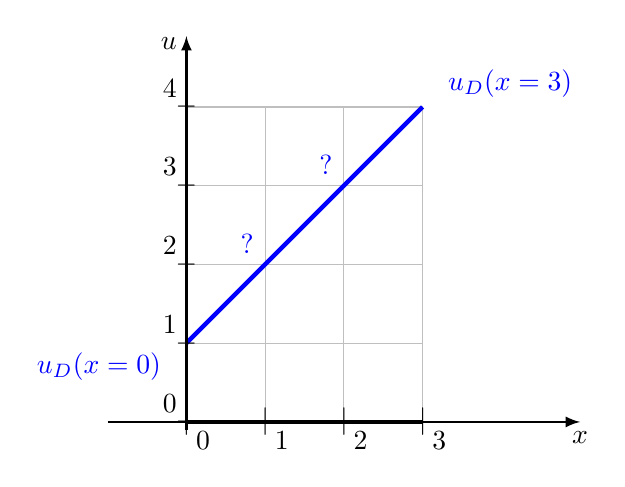
\begin{tikzpicture}[scale=1]

	% GRAPHE #1
    \begin{scope}
		\pgfmathsetmacro{\ox}{0};
		\pgfmathsetmacro{\ca}{1};
		%\pgfmathsetmacro{\cb}{1};

        %\clip (\ox-3,-2) rectangle (\ox+5,4);
        %grille    
    	\draw[thin, gray!50] (\ox,0) grid[step=1] ++(3,4);
    	% fct
        %\draw[thick, blue] plot[domain=-1:0] ({\ox+\x, \ca*\x+\cb});
        \draw[ultra thick, blue] plot[domain=0:3] ({\ox+\x, \ca*\x+1});
    
        %axes
        \draw[thick,->, >=latex] (\ox-1,0) -- ++(6,0);
        \draw[thick,->, >=latex] (\ox,-0.1) -- ++(0,5);
        \draw (\ox+5,0) node[anchor=north] {$x$};
        \draw (\ox+0,5) node[anchor=north east] {$u$};
    	% annotations    
    	%\draw[blue] (\ox-2,1.) node[anchor=north] {$E_1(x)$};

    \foreach \x in {0,...,3}
    {
        \draw (\x,0) node[below right] {\x};
        \draw (\x,0) node {$|$};
        \draw (\x,0) node {$\blacksquare$};

    }
    \foreach \x in {0,...,4}
    {
        \draw (0,\x) node[above left] {\x};
        \draw (0,\x) node {$-$};
    }
	\draw[ultra thick] (0,0) -- ++(3,0);
    \draw[ultra thick, blue] (0,1) node {$\square$} ;
    \draw[ultra thick, blue] (1,2) node {$\square$} node[above left] {$?$};
    \draw[ultra thick, blue] (2,3) node {$\square$} node[above left] {$?$} ;
    \draw[ultra thick, blue] (3,4) node {$\square$} ;

	\draw[blue] (-0.2,1) node[below left] {$u_D(x=0)$} ;
	\draw[blue] (3.2,4) node[above right] {$u_D(x=3)$} ;

	\end{scope}

\end{tikzpicture}

\end{center}

\end{slide}


%-----------------------------------------------------------------------
\begin{slide}[toc=]{Exemple simple}
%-----------------------------------------------------------------------

Vérifions que la méthode des éléments finis permet d'obtenir la solution analytique qui est linéaire ($u(x) = 1+x$).

\bigskip

L'assemblage des matrices élémentaires donne le système:

\begin{equation*}
\begin{bmatrix}
        1 & -1 &  0  & 0    \\
        -1 & 2 &  -1 & 0    \\
        0 & -1 & 2   & -1    \\
       0 & 0 &  -1 & 1    \\
    \end{bmatrix}
     \begin{bmatrix}
        u_1    \\
        u_2    \\
        u_3    \\
       u_4    \\
    \end{bmatrix}
    =
     \begin{bmatrix}
        0    \\
        0    \\
        0    \\
       0    \\
    \end{bmatrix}
\end{equation*}

Le système est tridiagonal.


\end{slide}



%-----------------------------------------------------------------------
\begin{slide}[toc=]{Exemple simple}
%-----------------------------------------------------------------------


En introduisant les conditions aux limites:

\begin{equation*}
\begin{bmatrix}
        \red\boldsymbol{1} & \red\boldsymbol{0} &  0  & 0    \\
        -1 & 2 &  -1 & 0    \\
        0 & -1 & 2   & -1 \\
       0 & 0 &  \red\boldsymbol{0} & \red\boldsymbol{1}    \\
    \end{bmatrix}
     \begin{bmatrix}
        u_1    \\
        u_2    \\
        u_3    \\
       u_4    \\
    \end{bmatrix}
    =
     \begin{bmatrix}
        \red\boldsymbol{1}    \\
        0    \\
        0    \\
       \red\boldsymbol{4}    \\
    \end{bmatrix}
\end{equation*}

\bigskip

En résolvant ce système on obtient $u_2=2$ et $u_3=3$ qui est la solution exacte du problème.

\bigskip

Remarquons que, dans ce cas très simple, le système d'équations EF obtenu est identique à celui qui aurait été obtenu par la méthode des différences finies.



\end{slide}




%=======================================================================
\section[toc=Exemple: EF 3D]{Exemple: Éléments Finis 3D}
%=======================================================================


%-----------------------------------------------------------------------
\begin{slide}{Cas de Laplace}
%-----------------------------------------------------------------------

La procédure est tout à fait identique à 3D.

\bigskip

Considérons à nouveau le problème de Laplace avec conditions aux limites de Dirichlet. L'approximation de Galerkin s'écrit:

\begin{equation*}
      \int_{\Omega} \boldsymbol{\nabla} h^* \cdot \boldsymbol{\nabla} u^* \,d\Omega
     =
     0
\end{equation*}
avec
\begin{equation*}
     u^*(\boldsymbol{x}) = \sum_{j=1}^N u_j \,\varphi_j(\boldsymbol{x})
\end{equation*}
\begin{equation*}
     h^*(\boldsymbol{x}) = \sum_{i=1}^N h_i \,\varphi_i(\boldsymbol{x})
\end{equation*}

\end{slide}



%-----------------------------------------------------------------------
\begin{slide}[toc=]{Cas de Laplace}
%-----------------------------------------------------------------------

En remplaçant $u^*$ et $h^*$ on obtient:
\begin{equation*}
    \sum_{i=0}^N \left[ \sum_{j=0}^N\underbrace{\left( \int_{\Omega} \boldsymbol{\nabla} \varphi_i(\boldsymbol{x})\cdot
    \boldsymbol{\nabla} \varphi_j(\boldsymbol{x})  \, d\Omega \right)}_{K_{ij}} \, u_j \right] \,  h_i
     = 0
\end{equation*}
c'est-à-dire
\begin{equation*}
    [K] \boldsymbol{u} = 0
\end{equation*}
qui est le même système qu'à 1D, où cette fois:
\begin{equation*}
    K_{ij} = \int_{\Omega} \boldsymbol{\nabla} \varphi_i(\boldsymbol{x})\cdot
    \boldsymbol{\nabla} \varphi_j(\boldsymbol{x})  \, d\Omega
\end{equation*}

\bigskip

Si on a $N_e$ éléments finis, l'intégrale sur le domaine $\Omega$ va être calculée comme la somme des intégrales sur chaque élément.
\begin{equation*}
    K_{ij} = \int_{\Omega} (\star)  \, d\Omega
    = \sum_{e=1}^{N_e} \left( \int_{E_e} (\star)  \, d\Omega \right)
    = \sum_{e=1}^{N_e} K^e_{ij}
\end{equation*}

\end{slide}




%-----------------------------------------------------------------------
\begin{slide}{Choix des $\varphi_k$}
%-----------------------------------------------------------------------


Imaginons que l'on maille le domaine $\Omega$ avec des hexaèdres.

\bigskip

Calculer la matrice $[K]$ du problème (dimension $N\times N$) revient à calculer la matrice $[K^e]$ de chaque hexaèdre (dimension $8\times 8$) et de sommer toutes les contributions via l'opération d'assemblage décrite précédemment.

\bigskip

Les fonctions $\varphi_k(\boldsymbol{x})$ choisies sont des fonctions trilinéaires (extension directe du cas 1D).

$\varphi_k$ vaut donc 1 au noeud $k$ et vaut 0 au autres noeuds.

\bigskip

    \centerline{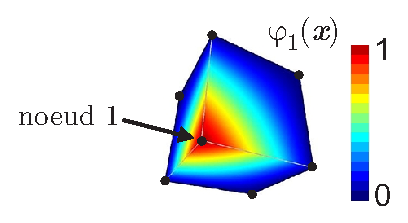
\includegraphics[width=0.5\textwidth]{phi3d.eps} }

\end{slide}


%-----------------------------------------------------------------------
\begin{slide}[toc=]{Choix des $\varphi_k$}
%-----------------------------------------------------------------------

Tout comme dans le cas 1D, on ne travaille que sur 1 élément à la fois. On effectue un changement de variables $\boldsymbol{x}=(x,y,z) \rightarrow \boldsymbol{\xi}=(\xi,\eta,\zeta)$ avec $\xi\in[-1,1]$, $\eta\in[-1,1]$, $\zeta\in[-1,1]$

    \centerline{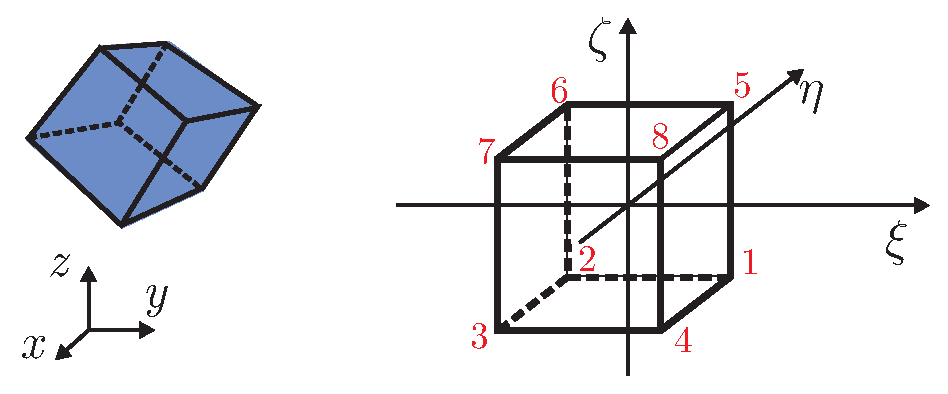
\includegraphics[width=0.8\textwidth]{hexa.eps} }

La volume d'un hexaèdre donné peut être paramétré en fonction de la position de ses noeuds ($\boldsymbol{x}_i$) grâce aux fonctions d'interpolation $\varphi_i$.

\begin{equation*}
    \boldsymbol{x}(\boldsymbol{\xi}) = \sum_{i=1}^8 \varphi_i(\boldsymbol{\xi}) \boldsymbol{x}_i
\end{equation*}

\end{slide}



%-----------------------------------------------------------------------
\begin{slide}[toc=]{Choix des $\varphi_k$}
%-----------------------------------------------------------------------

On définit:
\begin{equation*}
    \left\{
        \begin{aligned}
            &\varphi_1(\xi,\eta,\zeta) = \frac{1}{8} (1+\xi) (1+\eta) (1-\zeta) \\
            &\varphi_2(\xi,\eta,\zeta) = \frac{1}{8} (1-\xi) (1+\eta) (1-\zeta) \\
            &\varphi_3(\xi,\eta,\zeta) = \frac{1}{8} (1-\xi) (1-\eta) (1-\zeta) \\
            &\varphi_4(\xi,\eta,\zeta) = \frac{1}{8} (1+\xi) (1-\eta) (1-\zeta) \\
            &\varphi_5(\xi,\eta,\zeta) = \frac{1}{8} (1+\xi) (1+\eta) (1+\zeta) \\
            &\varphi_6(\xi,\eta,\zeta) = \frac{1}{8} (1-\xi) (1+\eta) (1+\zeta) \\
            &\varphi_7(\xi,\eta,\zeta) = \frac{1}{8} (1-\xi) (1-\eta) (1+\zeta) \\
            &\varphi_8(\xi,\eta,\zeta) = \frac{1}{8} (1+\xi) (1-\eta) (1+\zeta) \\
        \end{aligned}
    \right.
\end{equation*}

\end{slide}



%-----------------------------------------------------------------------
\begin{slide}[toc=Chgt de variables]{Changement de variables}
%-----------------------------------------------------------------------

Pour changer de variables, il est nécessaire de calculer le jacobien:
\begin{equation*}
     \begin{bmatrix}
\frac{\partial}{\partial\xi} \\
\frac{\partial}{\partial\eta} \\
\frac{\partial}{\partial\zeta} \\
    \end{bmatrix}
=
     \begin{bmatrix}
\frac{\partial x}{\partial\xi} & \frac{\partial y}{\partial\xi} & \frac{\partial z}{\partial\xi}   \\
\frac{\partial x}{\partial\eta} & \frac{\partial y}{\partial\eta} & \frac{\partial z}{\partial\eta}   \\
\frac{\partial x}{\partial\zeta} & \frac{\partial y}{\partial\zeta} & \frac{\partial z}{\partial\zeta}   \\
    \end{bmatrix}
     \begin{bmatrix}
\frac{\partial}{\partial x} \\
\frac{\partial}{\partial y} \\
\frac{\partial}{\partial z} \\
    \end{bmatrix}
       = [J]
            \begin{bmatrix}
\frac{\partial}{\partial x} \\
\frac{\partial}{\partial y} \\
\frac{\partial}{\partial z} \\
    \end{bmatrix}
\end{equation*}

c'est-à-dire

\begin{equation*}
     \begin{bmatrix}
\frac{\partial}{\partial\xi} \\
\frac{\partial}{\partial\eta} \\
\frac{\partial}{\partial\zeta} \\
    \end{bmatrix}
=
     \begin{bmatrix}
\sum_i \frac{\partial \varphi_i}{\partial\xi}x_i & \sum_i \frac{\partial \varphi_i}{\partial\xi}y_i & \sum_i \frac{\partial \varphi_i}{\partial\xi}z_i   \\
\sum_i \frac{\partial \varphi_i}{\partial\eta}x_i & \sum_i \frac{\partial \varphi_i}{\partial\eta}y_i & \sum_i \frac{\partial \varphi_i}{\partial\eta}z_i   \\
\sum_i \frac{\partial \varphi_i}{\partial\zeta}x_i & \sum_i \frac{\partial \varphi_i}{\partial\zeta}y_i & \sum_i \frac{\partial \varphi_i}{\partial\zeta}z_i   \\
    \end{bmatrix}
     \begin{bmatrix}
\frac{\partial}{\partial x} \\
\frac{\partial}{\partial y} \\
\frac{\partial}{\partial z} \\
    \end{bmatrix}
       = [J]
            \begin{bmatrix}
\frac{\partial}{\partial x} \\
\frac{\partial}{\partial y} \\
\frac{\partial}{\partial z} \\
    \end{bmatrix}
\end{equation*}

En notation compacte:
\begin{equation*}
\frac{\partial}{\partial \boldsymbol{\xi}} = [J] \frac{\partial}{\partial \boldsymbol{x}}
\qquad \Rightarrow \qquad
\frac{\partial}{\partial \boldsymbol{x}} = [J]^{-1} \frac{\partial}{\partial \boldsymbol{\xi}}
\end{equation*}
Le rapport des volumes est le déterminant du jacobien:
\begin{equation*}
d\Omega = dx\,dy\,dz = \det [J] \, d\xi\,d\eta\,d\zeta
\end{equation*}

\end{slide}


%-----------------------------------------------------------------------
\begin{slide}{Calcul de $K^e$}
%-----------------------------------------------------------------------

La composante $i,j$ de la matrice élémentaire $[K^e]$ s'écrit:

\begin{equation*}
    K^e_{ij} = \int_{E^e} \boldsymbol{\nabla} \varphi_i(\boldsymbol{x})\cdot
    \boldsymbol{\nabla} \varphi_j(\boldsymbol{x})  \, dx\,dy\,dz
\end{equation*}

qui devient, après changement de variables:
\begin{equation*}
    K^e_{ij} = \int_{-1}^1\int_{-1}^1\int_{-1}^1 [J]^{-1} \boldsymbol{\nabla}_{\xi} \varphi_i(\boldsymbol{\xi})\cdot
    [J]^{-1} \boldsymbol{\nabla}_{\xi} \varphi_j(\boldsymbol{\xi})  \, \det [J] \, d\xi\,d\eta\,d\zeta
\end{equation*}

\bigskip

De manière plus compacte:
\begin{equation*}
    K^e_{ij} = \int_{-1}^1\int_{-1}^1\int_{-1}^1 J_{km}^{-1} \frac{\partial\varphi_i}{\xi_m}
    J_{kn}^{-1} \frac{\partial\varphi_j}{\xi_n}  \, \det [J] \, \xi_1\,d\xi_2\,d\xi_3
\end{equation*}
où on a noté $(\xi, \eta, \zeta)=(\xi_1, \xi_2, \xi_3)$.

\end{slide}



%-----------------------------------------------------------------------
\begin{slide}[toc=]{Exemple}
%-----------------------------------------------------------------------

Imaginons un hexaèdre alignés sur les axes dont le jacobien vaut 1. Dans ce cas, la matrice $K^e$ peut être évaluée analytiquement. On obtient~:

\begin{equation*}
[K^e]=
     \begin{bmatrix}
 \frac{2}{3}&     0      &-\frac{1}{6}&  0         &    0       &-\frac{1}{6}&-\frac{1}{6}&-\frac{1}{6}   \\
     0      &\frac{2}{3} &     0      &-\frac{1}{6}&-\frac{1}{6}&0           &-\frac{1}{6}&-\frac{1}{6}   \\
-\frac{1}{6}&0           &\frac{2}{3} &     0      &-\frac{1}{6}&-\frac{1}{6}&0           &-\frac{1}{6}   \\
0           &-\frac{1}{6}&0           &\frac{2}{3} &-\frac{1}{6}&-\frac{1}{6}&-\frac{1}{6}&0              \\
0           &-\frac{1}{6}&-\frac{1}{6}&-\frac{1}{6}&\frac{2}{3} & 0          &-\frac{1}{6}&0              \\
-\frac{1}{6}&0           &-\frac{1}{6}&-\frac{1}{6}&0           &\frac{2}{3} &0           &-\frac{1}{6}   \\
-\frac{1}{6}&-\frac{1}{6}&0           &-\frac{1}{6}&-\frac{1}{6}&0           &\frac{2}{3} &0              \\
-\frac{1}{6}&-\frac{1}{6}&-\frac{1}{6}&0           & 0          &-\frac{1}{6}&0           &\frac{2}{3}    \\
    \end{bmatrix}
\end{equation*}

\bigskip

Ce résultat est utile pour vérifier un code élément fini!

\end{slide}



%=======================================================================
\section{Intégration de Gauss}
%=======================================================================

%-----------------------------------------------------------------------
\begin{slide}{Rappel}
%-----------------------------------------------------------------------

Mis à part pour le cas 1D, évaluer analytiquement les intégrales apparaissant dans l'expression des matrices des éléments finis n'est pas possible analytiquement.

On utilise donc une méthode numérique d'intégration (quadrature de Gauss).

\bigskip

\emph{Cas 1D}

\begin{equation*}
    \int_{-1}^1 f(\xi) \,d\xi \approx \sum_{i=1}^p w_i\, f(\xi_i)
\end{equation*}
où
\begin{itemize}
    \item $p$ est le nombre de points d'intégration
    \item $w_i$ sont les poids d'intégration
    \item $\xi_i$ sont les positions des points d'intégration.
\end{itemize}

Une intégration de Gauss avec $p$ points permet d'intégrer exactement des polynômes de degré $2p-1$.

\end{slide}


%-----------------------------------------------------------------------
\begin{slide}[toc=]{Rappel}
%-----------------------------------------------------------------------

Position des points et valeurs des poids

\begin{center}
\begin{tabular}{|c|c|c|c|}
  \hline
  % after \\: \hline or \cline{col1-col2} \cline{col3-col4} ...
  $p$  & $\xi_1$ & $\xi_2$ & $\xi_3$ \\ \hline
  1 & 0 & - & - \\
  2 & $-1/\sqrt{3}$ & $1/\sqrt{3}$ & - \\
  3 & $-\sqrt{3/5}$ & 0 & $\sqrt{3/5}$ \\
  \hline
\end{tabular}
\end{center}


\begin{center}
\begin{tabular}{|c|c|c|c|}
  \hline
  % after \\: \hline or \cline{col1-col2} \cline{col3-col4} ...
  $p$  & $w_1$ & $w_2$ & $w_3$ \\ \hline
  1 & 2 & - & - \\
  2 & 1 & 1 & - \\
  3 & $5/9$ & $8/9$ & $5/9$ \\
  \hline
\end{tabular}
\end{center}

\end{slide}





%-----------------------------------------------------------------------
\begin{slide}{Cas 3D}
%-----------------------------------------------------------------------

Pour les hexaèdres développés ici, on a 3 intégrales. On utilisera donc~:

\begin{equation*}
    \int_{-1}^1\int_{-1}^1\int_{-1}^1 f(\xi,\eta,\zeta) \,d\xi\,d\eta\,d\zeta
    \approx
    \sum_{i=1}^p\sum_{j=1}^p\sum_{k=1}^p
    w_i\,w_j\,w_k\, f(\xi_i,\xi_j,\xi_k)
\end{equation*}
On utilise le même nombre de points dans chaque direction de l'espace.

\bigskip

En pratique, 2 points suffisent dans chaque direction.
On utilise $2\times 2\times 2=8$ points de Gauss par élément fini.

\end{slide}








%=======================================================================
\section{Implémentation}
%=======================================================================

%-----------------------------------------------------------------------
\begin{slide}[method=file, toc=gmm++]{Objets Matrices/Vecteurs: gmm++}   % method=file pour "lstinputlisting"
%-----------------------------------------------------------------------

Manipuler des matrices et des vecteurs en C peut être fastidieux. On propose d'utiliser la bibliothèque
\href{http://download.gna.org/getfem/html/homepage/gmm/}{gmm++} qui facilitera grandement le travail.

\bigskip

Documentation \href{http://download.gna.org/getfem/html/homepage/userdoc/index.html}{en ligne}.

\bigskip

Mise en route:
\begin{itemize}
\item décomprimez \href{http://download.gna.org/getfem/stable/gmm-4.2.tar.gz}{gmm-4.2.tar.gz} dans votre répertoire de sources
\item ajoutez cette ligne dans vos fichiers sources:
\lstinputlisting{lst/include_gmm.cpp}
\item modifiez votre {\tt CMakeLists.txt}:
\lstinputlisting{lst/cmake_gmm.txt}
\end{itemize}

\bigskip
Remarque: pas besoin de compiler gmm++: c'est une bibliothèque de templates (tout est codé dans des fichiers {\tt .h}).


\end{slide}

%-----------------------------------------------------------------------
\begin{slide}[method=file, toc=Vecteurs]{Vecteurs gmm++}  %method=file pour "verb"
%-----------------------------------------------------------------------

gmm++ est compatible avec \verb$std::vector<double>$.

\lstinputlisting{lst/vectoradd_gmm.cpp}
Résultat:
\lstinputlisting{lst/vectoradd_gmm.txt}

\end{slide}


%-----------------------------------------------------------------------
\begin{slide}[method=file, toc=]{Vecteurs gmm++}  %method=file pour "verb"
%-----------------------------------------------------------------------

\emph{Exemples d'opérations sur des vecteurs:}

\bigskip

\begin{tabular}{l|l}
  % after \\: \hline or \cline{col1-col2} \cline{col3-col4} ...
  $\boldsymbol{v}_2\leftarrow\boldsymbol{v}_2+\boldsymbol{v}_1$      & \verb$gmm::add(v1, v2)$ \\
  $\boldsymbol{v}_2\leftarrow\, 2\,\boldsymbol{v}_2+\boldsymbol{v}_1$  & \verb$gmm::add(v1, gmm::scaled(v2,2.0), v_2)$\\
  $\boldsymbol{v}_1\leftarrow 2\,\boldsymbol{v}_1$         & \verb$gmm::scale(v1,2.0)$  \\
  $ s = \boldsymbol{v}_1\cdot \boldsymbol{v}_2$             & \verb$double s = gmm::vect_sp(v1, v2)$\\
  $ v_1 = 0$                                                & \verb$gmm::clear(v1)$ \\
  $ v_1 = v_2$                                              & \verb$gmm::copy(v2, v1)$ \\
  $ s = ||v_1||$                                            & \verb$double s = gmm::vect_norm2(v1)$ \\
\end{tabular}

\bigskip

\begin{itemize}
\item Accès aux éléments: opérateur \verb$[i]$
\item Taille du vecteur: \verb$gmm::vect_size(v)$
\end{itemize}

\vspace{\stretch{1}}

Lisez la \href{http://download.gna.org/getfem/html/homepage/userdoc/index.html}{doc en ligne}!

\end{slide}

%-----------------------------------------------------------------------
\begin{slide}[method=file, toc=Matrices pleines]{Matrices pleines gmm++}  %method=file pour "verb"
%-----------------------------------------------------------------------

gmm++ définit \verb$std::dense_matrix<double>$.

\lstinputlisting{lst/matrixadd_gmm.cpp}
Résultat:
\lstinputlisting{lst/matrixadd_gmm.txt}

\end{slide}


%-----------------------------------------------------------------------
\begin{slide}[method=file, toc=]{Matrices pleines gmm++}  %method=file pour "verb"
%-----------------------------------------------------------------------

\emph{Exemples d'opérations sur des matrices:}

\bigskip

\begin{tabular}{l|l}
  % after \\: \hline or \cline{col1-col2} \cline{col3-col4} ...
  $[A]=[A]+[B]$                                             & \verb$gmm::add(B, A)$ \\
  $[A]=[B] [C]$                                             & \verb$gmm::mult(B, C, A)$\\
  $\boldsymbol{v}_2\leftarrow\boldsymbol{v}_2+[A] \boldsymbol{v}_1$ & \verb$gmm::mult_add(A, v1, v2)$\\
  $ [A] = 0$                                                & \verb$gmm::clear(A)$ \\
  $ [A] = [B]$                                              & \verb$gmm::copy(B, A)$ \\
  $ s = ||A||_{\max}$                                       & \verb$double s = gmm::mat_maxnorm(A)$ \\
  $ s = \text{trace} [A]$                                   & \verb$double s = gmm::mat_trace(A)$ \\
  $ s = \text{det} [A]$                                     & \verb$double s = gmm::lu_det(A)$ \\
  $ [A]\rightarrow [A]^{-1}$                                & \verb$gmm::lu_inverse(A)$ \\
\end{tabular}

\bigskip

\begin{itemize}
\item Accès aux éléments: opérateur \verb$(i,j)$
\item Taille de la matrice: \verb$gmm::mat_nrows(A)$ et \verb$gmm::mat_ncols(A)$
\end{itemize}

\vspace{\stretch{1}}


Lisez la \href{http://download.gna.org/getfem/html/homepage/userdoc/index.html}{doc en ligne}!

\end{slide}


%-----------------------------------------------------------------------
\begin{slide}[method=file]{Calcul de $K^e$}  %method=file pour "verb"
%-----------------------------------------------------------------------

Pour rappel, la matrice $K^e$ s'écrit:
\begin{equation*}
    K^e_{ij} = \int_{-1}^1\int_{-1}^1\int_{-1}^1 [J]^{-1} \boldsymbol{\nabla}_{\xi} \varphi_i(\boldsymbol{\xi})\cdot
    [J]^{-1} \boldsymbol{\nabla}_{\xi} \varphi_j(\boldsymbol{\xi})  \, \det [J] \, d\xi\,d\eta\,d\zeta
\end{equation*}

\bigskip
Pour chaque $(i,j)$, l'intégrale est calculée sur $p^3$ points de Gauss
\begin{equation*}
    K^e_{ij} = \sum_{\alpha=1}^p\sum_{\beta=1}^p\sum_{\gamma=1}^p
    w_{\alpha}\,w_{\beta}\,w_{\gamma}\, f(\xi_1^{\alpha},\xi_2^{\beta},\xi_3^{\gamma})
\end{equation*}
avec
\begin{equation*}
    f(\xi_1^{\alpha},\xi_2^{\beta},\xi_3^{\gamma}) =
    \left[
    [J]^{-1} \boldsymbol{\nabla}_{\xi} \varphi_i(\boldsymbol{\xi})\cdot
    [J]^{-1} \boldsymbol{\nabla}_{\xi} \varphi_j(\boldsymbol{\xi})  \, \det [J]
    \right]_{\boldsymbol{\xi}=(\xi_1^{\alpha},\xi_2^{\beta},\xi_3^{\gamma})}
\end{equation*}
\begin{equation*}
    =
    \left[
    \begin{bmatrix}
    J_{11}^{-1}  & J_{12}^{-1} & J_{13}^{-1}  \\
    J_{21}^{-1}  & J_{22}^{-1} & J_{23}^{-1}  \\
    J_{31}^{-1}  & J_{32}^{-1} & J_{33}^{-1}  \\
    \end{bmatrix}
    \begin{bmatrix}
    \frac{\partial\varphi^i}{\partial\xi_1}   \\
    \frac{\partial\varphi^i}{\partial\xi_2}   \\
    \frac{\partial\varphi^i}{\partial\xi_3}   \\
    \end{bmatrix}
    \cdot
    \begin{bmatrix}
    J_{11}^{-1}  & J_{12}^{-1} & J_{13}^{-1}  \\
    J_{21}^{-1}  & J_{22}^{-1} & J_{23}^{-1}  \\
    J_{31}^{-1}  & J_{32}^{-1} & J_{33}^{-1}  \\
    \end{bmatrix}
    \begin{bmatrix}
    \frac{\partial\varphi^j}{\partial\xi_1}   \\
    \frac{\partial\varphi^j}{\partial\xi_2}   \\
    \frac{\partial\varphi^j}{\partial\xi_3}   \\
    \end{bmatrix}
\, \det [J]
    \right]_{\boldsymbol{\xi}=\boldsymbol{\xi}^{\alpha,\beta,\gamma} }
\end{equation*}

\end{slide}



%-----------------------------------------------------------------------
\begin{slide}[method=file,toc=]{Calcul de $K^e$}  %method=file pour "verb"
%-----------------------------------------------------------------------

Algorithme d'évaluation (non optimisé):

\bigskip

\noindent\fbox{\parbox{\linewidth-2\fboxrule-2\fboxsep}{ %-----------------------------------------------------------
\emph{Calcul de $K^e$}
\begin{itemize}
\item Boucle sur les points de Gauss $(\alpha=1\ldots p;\beta=1\ldots p;\gamma=1\ldots p)$
    \begin{itemize}
        \item Calcul de $[J]$ et de son déterminant en $(\xi_1^{\alpha},\xi_2^{\beta},\xi_3^{\gamma})$
        \item Calcul de $[J]^{-1}$.
        \item Boucle sur $(i,j)$ :
        \begin{itemize}
            \item Calcul des vecteurs $\boldsymbol{\nabla}_{\boldsymbol{\xi}}\varphi_i$ et $\boldsymbol{\nabla}_{\boldsymbol{\xi}}\varphi_i$
            \item Calcul de $[J^{-1}] \boldsymbol{\nabla}_{\boldsymbol{\xi}}\varphi_i$ et $[J^{-1}] \boldsymbol{\nabla}_{\boldsymbol{\xi}}\varphi_j$.
            \item Calcul de $f_{ij}(\xi_1^{\alpha},\xi_2^{\beta},\xi_3^{\gamma})$ par produit scalaire des 2 résultats et multiplication par $\det [J]$.
            \item $K^e_{ij} \leftarrow K^e_{ij} + (w_{\alpha}\,w_{\beta}\,w_{\gamma}) \, f_{ij}(\xi_1^{\alpha},\xi_2^{\beta},\xi_3^{\gamma})$
        \end{itemize}
    \end{itemize}
\end{itemize}
}} %-----------------------------------------------------------------------------------------------------------------

\end{slide}


%-----------------------------------------------------------------------
\begin{slide}[method=file,toc=]{Calcul de $K^e$}  %method=file pour "verb"
%-----------------------------------------------------------------------

Conseil: Toujours obtenir d'abord un code qui fonctionne avant de penser à l'optimisation!

\bigskip

Quelques optimisations possibles:
\begin{itemize}
\item La matrice $K^e$ est symétrique...
\item Il est possible de précalculer certaines grandeurs telles que $\varphi_i(\xi_{\alpha},\xi_{\beta},\xi_{\gamma})$ et ses dérivées spatiales.
\item On peut sortir le facteur $(w_{\alpha}\,w_{\beta}\,w_{\gamma})\det [J]$ de la boucle interne $(i,j)$.
\item Calcul simultané de plusieurs $K^e$ (parallélisation).
\item Si l'équation de départ est plus complexe, plusieurs matrices doivent être calculées (une pour chaque terme). Ces matrices font intervenir des facteurs similaires qui peuvent être réutilisés d'une matrice à l'autre.
\item etc.
\end{itemize}


\end{slide}


%-----------------------------------------------------------------------
\begin{slide}[method=file,toc=Matrices creuses]{Matrices creuses}  %method=file pour "verb"
%-----------------------------------------------------------------------

La matrice $[K]$ résulte de l'assemblage des matrices $[K^e]$ comme expliqué précédemment. Elle est très creuse (très peu d'éléments non nuls).

    \centerline{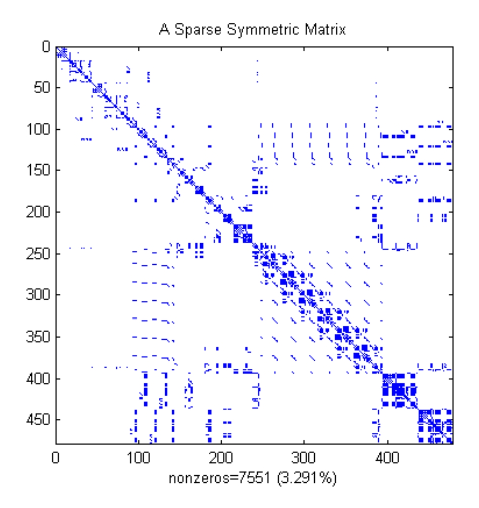
\includegraphics[width=0.3\textwidth]{sparse.eps} }

Cette propriété doit être prise en compte dans un code EF pour des questions d'efficacité et de mémoire.

\bigskip

Un format creux courant est le \href{http://en.wikipedia.org/wiki/Sparse_matrix}{format CSR} (Compressed Sparse Row). Il est utilisé par de nombreux solveurs linéaires.

\end{slide}


%-----------------------------------------------------------------------
\begin{slide}[method=file,toc=]{Matrices creuses gmm++}  %method=file pour "verb"
%-----------------------------------------------------------------------

\emph{Implémentation:} gmm++ propose \verb$gmm::csr_matrix<double>$.

\bigskip

Subtilité: ce type optimisé de matrices ne peut être utilisé qu'en lecture. On doit donc utiliser un autre type lors de l'assemblage:

\bigskip

\lstinputlisting{lst/assembly.cpp}

\end{slide}



%-----------------------------------------------------------------------
\begin{slide}[method=file,toc=Solveur linéaire]{Résoudre le système}  %method=file pour "verb"
%-----------------------------------------------------------------------

gmm++ propose plusieurs solveurs linéaires:
\begin{itemize}
\item Un solveur LU: \verb$gmm::lu_solve()$
\item Des solveurs itératifs (GMRES, CG, etc.): \verb$gmm::gmres()$
\item Une interface avec \href{http://crd-legacy.lbl.gov/~xiaoye/SuperLU/}{SuperLU}: \verb$gmm::SuperLU_solve()$
\item Une interface avec \href{http://mumps.enseeiht.fr/}{MUMPS}: \verb$gmm::MUMPS_solve()$
\end{itemize}


\end{slide}



%-----------------------------------------------------------------------
\begin{slide}[method=file,toc=]{Interface gmm/MUMPS}  %method=file pour "verb"
%-----------------------------------------------------------------------

Installez MUMPS dans la Virtualbox jean/valjean:

%\verb$sudo apt-get install libmumps-dev$
\begin{center}
\verb$sudo apt-get install libmumps-seq-dev$
\end{center}

\bigskip
Adaptez votre \verb$CMakeLists.txt$:

\lstinputlisting{lst/cmake_mumps.txt}

\end{slide}



%-----------------------------------------------------------------------
\begin{slide}[method=file,toc=]{Interface gmm/MUMPS}  %method=file pour "verb"
%-----------------------------------------------------------------------

Programme de test:

\lstinputlisting{lst/testMUMPS_1.cpp}

\end{slide}



%-----------------------------------------------------------------------
\begin{slide}[method=file,toc=]{Interface gmm/MUMPS}  %method=file pour "verb"
%-----------------------------------------------------------------------

\lstinputlisting{lst/testMUMPS_2.cpp}

\bigskip
Accès au code: (projet \verb$femcode/mumps$)

\begin{center}
\verb$git clone https://github.com/rboman/femcode.git$
\end{center}

(ou \verb$git pull$ si vous avez déjà cloné \verb$femcode$)


\end{slide}


%-----------------------------------------------------------------------
\begin{slide}[method=file,toc=]{Interface gmm/MUMPS}  %method=file pour "verb"
%-----------------------------------------------------------------------

Résultats:

\lstinputlisting{lst/testMUMPS.txt}

\end{slide}







\end{document}




